%!TEX root = main.tex

\documentclass[main.tex]{subfiles}

\begin{document}

\chapter{Background}
In this chapter an introduction will be given to the theoretical framework of digital waveguides which form the basis for the synthesis model developed in this thesis. After these ideas have been covered, the slide guitar model which inspired this thesis will be outlined. A basic overview will be given with emphasis on the theoretical derivations as a more detailed analysis of the implementation will be covered in subsequent chapters. The chapter will conclude with an overview and comparison of the more recent approaches to slide guitar synthesis.

\section{Physical Modeling and Digital Waveguides}
Physical modeling is a discipline which attempts to recreate physical phenomena using computational algorithms \citetwo{smith_physical_nodate}. There are many different approaches to this, however one of the most popular and well developed is the technique of digital waveguides (DWG). As the name would imply, this approach uses algorithms and data structures to mimic the method by which waves propagate throughout a medium. It is an extremely computationally efficient technique that has been incorporated into many different commercial synthesizers.

\subsection{Fundamental Components}
Two of the fundamental components of digital waveguide models are digital filters and digital delay lines \citetwo{smith_physical_nodate}. The second component can be broken down into integer and fractional length delay lines. The interconnection of these different components models a variety of wave propagation phenomena. Through the incorporation of different noise sources and initialization waveforms, a large number of different sound synthesis algorithms can be created.

\subsubsection{Digital Filters}
Conceptually digital filters are extremely simple computational structures. They merely add scaled time-delayed versions of their inputs and outputs. Through various combinations of delay and scaling, a range of different frequency domain effects can be achieved. They are linear systems, which is useful as the entire branch of linear-time invariant (LTI) systems is now made available to the algorithm designer.

Digital filters come in two varieties: finite impulse response (FIR) and infinite impulse response (IIR). FIR filters consist of only delayed and scaled copies of the input signal while IIR filters incorporate the output of the filter via feedback connections. This is what gives rise to the ``infinite" aspect of their name as theoretically the feedback makes it so the filter's output in response to an impulse signal would never completely decay (ignoring the effects of digital arithmetic).

All filters exhibit a transient response \citetwo{oppenheim_signals_1997}. These occur whenever there is a change in the coefficients associated with a filter's structure as well as when the input changes from steady-state. FIR filters have a transient whose length corresponds to the order of the filter. IIR filters pose more of a problem with regards to transients as their feedback cause the transients to propagate for a much longer time (depending on the attenuation provided by the filter's coefficients). Figure~\ref{fig:generic_IIR} illustrates a generic IIR filter structure.

\begin{figure}[h]
    \centering
    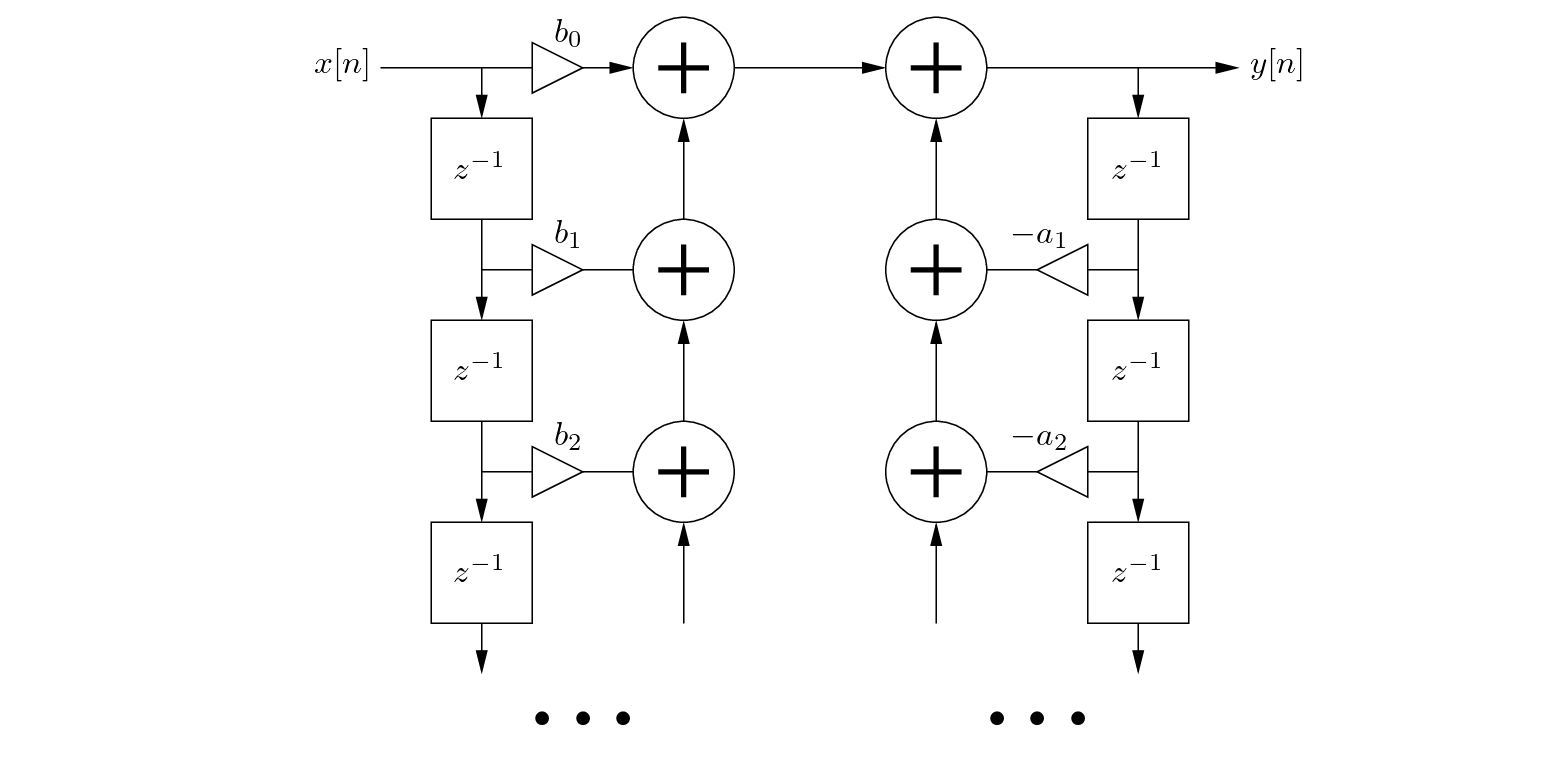
\includegraphics[scale=.25]{./images/diagrams/digitalFilter.png}
    \caption{A generic digital filter structure. The $b_n$ coefficients refer to the feedfoward part while the $a_n$ coefficients refer to the feedback part \citetwo{scavone_infinite_2023}. An FIR filter would consist of only the feedforard component.}
    \label{fig:generic_IIR}
\end{figure}

\subsubsection{Digital Delay Lines}
The digital delay line is one of the fundamental components of DWG based modeling \citetwo{scavone_digital_2023-1}. Its main purpose is to provide a computational model of the time delay experienced by waves propagating a particular medium. The digital values a delay line holds represent physical quantities as they evolve over time at spatially sampled locations of the physical medium. The physical distance between each spatial sample corresponds to the distance a wave travels during one sampling period. Mathematically, this can be expressed in the following equation:
\begin{equation}
    X_s = T_s \times c
\end{equation}
where $T_s$ is the temporal sampling period and $c$ is the wave propagation speed in the particular media being modeled \citetwo{scavone_sampled_2023}. Figure~\ref{fig:digitalDelayLine} illustrates a pictorial representation of a digital delay line (of $M$ samples) frequently used in signal processing diagrams.

Unfortunately, there is an inherent limitation to digital delay lines. This is due to the fact that the fundamental unit of discretization in the time-domain is the sample. This means that signals can only be delayed/modeled using integer numbers of samples with this structure. In many physical modeling applications, this is a problematic due to the fact that the physical world and its associated laws are not spatially quantized. It is often required to know a physical quantity which at a point which lies between two spatial samples.

\begin{figure}[h]
    \centering
    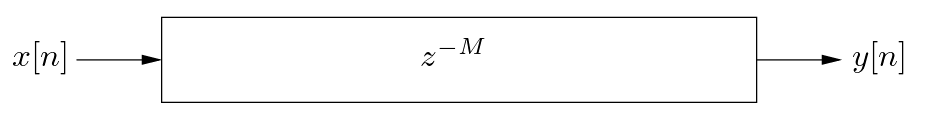
\includegraphics[scale=.25]{./images/diagrams/digitalDelayLine.png}
    \caption{Pictorial representation of a digital delay component which is $M$ samples in length \citetwo{scavone_digital_2023}.}
    \label{fig:digitalDelayLine}
\end{figure}

\subsubsection{Delay Line Interpolation}
Various approaches have been developed in an attempt to approximate the signal values in between samples of a digital delay line \citetwo{laakso_splitting_1996}. As a value is being determined which lies in between two known values, the task is fundamentally interpolation. The different interpolation approaches are implemented using filters whose coefficients are calculated in a particular way to achieve the desired degree of fractional/sub-sample approximation. When combined in series at the output of an integer delay line, the overall structure is referred to as a fractional delay line. Given the techniques are realized using filters, the different approaches have various frequency/time domain implications and transients can become an issue (in the case of a time-varying delay line length).

One popular approach to fractional delay line implementations is Lagrange interpolation. In this technique an FIR filter is used where the filter coefficients implement Largange interpolation to allow for sub-sample accuracy \citetwo{valimaki_discrete-time_1995}. Figure~\ref{fig:LagrangeStructure} illustrates the FIR filter in series with an $M$ sample delay line. The equation used to generate the coefficients is:
\begin{equation}
    h[n] = \prod_{k=0}^{N} \frac{D-k}{n-k}, \text{for } n=0, 1, ... N \text{ and } k \ne n
\end{equation}

The order of the filter determines the order of the polynomials involved following the theory of Lagrange interpolation. With an order of N = 1, linear interpolation is achieved. Adjusting the order of the filter allows you to have more control over its frequency response and phase delay. The Lagrange approach can generate a filter structure which has a constant phase delay under certain conditions. Figure~\ref{fig:LagrangeResponses} illustrates how the resulting filter has low-pass characteristics and can exhibit a constant phase delay under certain conditions.

\begin{figure}[h]
    \centering
    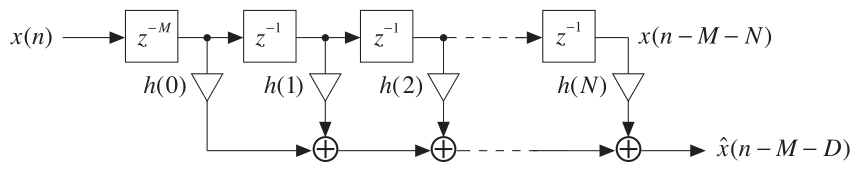
\includegraphics[scale=.65]{./images/diagrams/LagrangeStructure.png}
    \caption{An FIR structure implementing Lagrange interpolation in series with an $M$ sample delay line \citetwo{valimaki_discrete-time_1995}}
    \label{fig:LagrangeStructure}
\end{figure}

\begin{figure}[h]
    \centering
    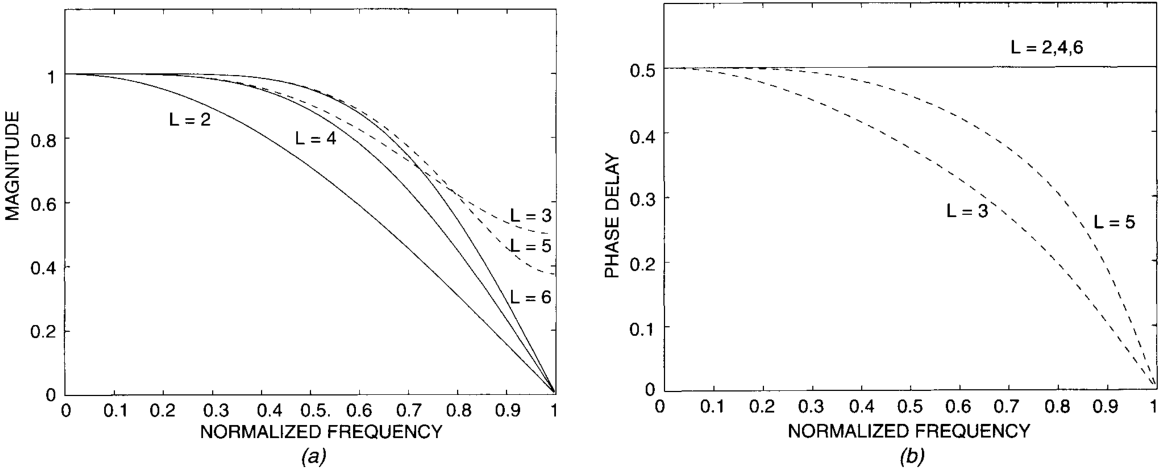
\includegraphics[scale=.65]{./images/plots/LagrangeResponses.png}
    \caption{a) Magnitude and b) phase delay responses of Lagrange interpolating filters of length L = 2, 3, 4, 5, and 6 with d = 0.5 \citetwo{laakso_splitting_1996}}
    \label{fig:LagrangeResponses}
\end{figure}

\subsection{Applied to String Modeling}
The wave equation can be used to derive the following general solution to wave motion in a string:
\begin{equation}
    y(x,t) = Ae^{j\left(\omega t \pm k x\right)}
\end{equation}
where $y(x,t)$ represents the transverse displacement, $A$ is the complex amplitude and $k$ is the wave number. d'Alembert reformulated this into another expression which can be interpreted as the sum of two identical waves traveling in opposite directions \citetwo{smith_physical_nodate}. It is:
\begin{equation}
    y(x,t) = y^{+}(ct - x) + y^{-}(ct + x)
\end{equation}
where $c$ is the wave speed and $y^+$ and $y^-$ represent a wave traveling in the positive and negative $x$ directions respectively, with the same speed. In the physical world, strings need to have a finite length and often have a termination at each end which is referred to as a load impedance. These impedances have their own effects in the frequency domain and can be considered as filters. When a traveling wave encounters of of the termination impedances, it is reflected back along the string to travel in the opposite direction with the frequency effects of the corresponding load impedance applied to it. 

If this was to be implemented via a DWG model, an initial approach would consist of a digital delay line representing each direction of propagation as well as a filter at each of the end of the string's terminations. Figure~\ref{fig:BiDirectionDWG} illustrates a signal flow diagram for this bi-directional computational model. The traveling wave variables could be any physical quantity related to the string movement (i.e. displacement, acceleration, velocity...) depending on what is desired for the synthesis model, however transverse displacement is commonly used for string models. This is because transverse vibrations are primarily how string instruments are played. In combination with the laws of physics and other physical quantities, like the characteristic impedance, it is easy to calculate the other physical aspects which might be needed. In the case of a guitar the terminations are the nut and the bridge.

Plucking a string corresponds to imparting an initial displacement along its length \citetwo{smith_physical_nodate}. For a DWG model, this corresponds to the waveform which is used to initialize digital delays when modeling the transverse displacement. The output, $y[n]$ can be determined at any spatial location by summing the appropriate spatial samples from each of the different traveling wave simulations (applying interpolation where is necessary). Determining where the output will be taken is part of the synthesis model. The bridge is commonly used as the output location for string models as this is where the vibrations of the string are transferred to the body of the instrument. The body's effects often create the distinguishing characteristics of a string instrument.

\begin{figure}[h]
    \centering
    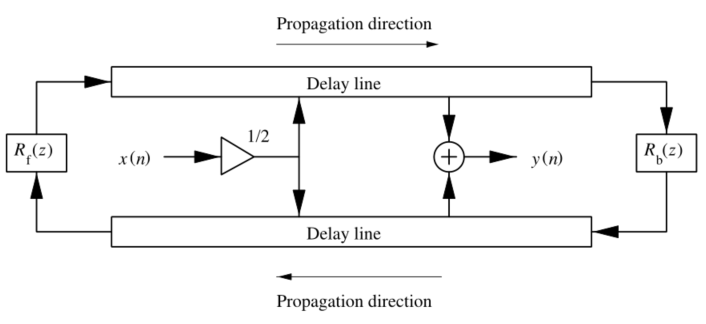
\includegraphics[scale=.85]{./images/diagrams/BiDirectionalDWG1.png}
    \caption{A bi-directional DWG structure for a string terminated at both ends \citetwo{karjalainen_plucked-string_1998}}
    \label{fig:BiDirectionDWG}
\end{figure}

By exploiting the linearity of the systems involved, as well as the fact that is generally only desired to know the output at one specific spatial location, it is possible to commute the different components of the bi-directional system into a substantially more efficient model. Figure~\ref{fig:SDLModel} illustrates this new computational structure, which is referred to as the single-delay loop (SDL) structure \citetwo{karjalainen_plucked-string_1998}. The various traveling losses and other effects from phenomena like reflection and dispersion have been combined into the loop filter $H_l(z)$. Additionally, it is no longer required to simulate both traveling waves so only one delay line is required (as the structure's name would imply).

\begin{figure}[h]
    \centering
    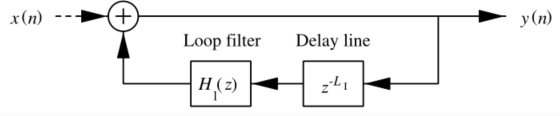
\includegraphics[scale=1]{./images/diagrams/SDLModel.png}
    \caption{A single delay line DWG structure for a string \citetwo{karjalainen_plucked-string_1998}}
    \label{fig:SDLModel}
\end{figure}

\subsubsection{Controlling Pitch}
Suppose you have a string of a given length which is vibrating. It will produce a pitch with a corresponding fundamental frequency $F_0$. This is referred to as the open string fundamental. If the length of the string is shortened, then the fundamental of the pitch will be scaled inversely proportional to the relative string length \citetwo{valimaki_development_1998}. If $L$ represents the relative string length, which exists on the interval $(0, 1]$, the fundamental at a specified relative string length can be expressed as:

\begin{equation}
    F_L = \frac{F_0}{L}
    \label{eq:F_L}
\end{equation}
This relationship is fundamental to the nature of how the guitar is played, with the frets traditionally determining the different values $L$ can take.

In terms of the DWG structure, controlling the physical length of the string equates to controlling the number of samples in the delay line. Supposing that $F_L$ and the sampling rate are known, the DWG length (in samples) can be calculated using the expression:
\begin{equation}
    \text{DWG Length} = \frac{F_s}{F_L}
\end{equation}

From this we can clearly see why it is necessary to use an interpolation method as described before. If the length of the digital wave guide is limited to purely integer values, then the fundamentals of the synthesized tones will be quantized to integer divisions of the sampling frequency. In order to have the synthesis model be more flexible, expressive, and usable, it is necessary to allow the digital wave guide length to take on non-integer values. This issue is well known in the literature as shown in \citetwo{jaffe_extensions_1983}.

\subsubsection{Determining DWG Length}
In order to express the length of the SDL structure, it is necessary to breakdown the delay line into its constituent components as shown in Fig.~\ref{fig:SDLBreakdown}. The total delay which a waveform propagating through the system will encounter, can be expressed as the sum of the phase delays of the components in the loop: 
\begin{equation}
    \text{DWG Length} = \tau_{H_L} + L_f + L_I
\end{equation}
where $\tau_{H_L}$ represents the phase delay of the loop filter, $L_f$ represents the phase delay of the filter implementing the fractional interpolation and $L_I$ represents the integer delay line length. These quantities can be either static or time-varying depending on the type of articulation and sound being synthesized \citetwo{karjalainen_plucked-string_1998}. This also highlights the importance of the loop filter and fractional approximation method used in the model.

\begin{figure}[h]
    \centering
    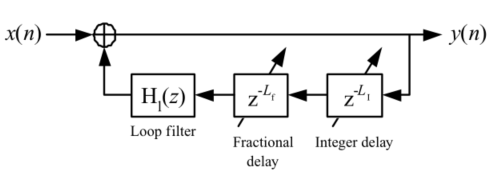
\includegraphics[scale=1]{./images/diagrams/SDLModelExpanded.png}
    \caption{SDL expanded \citetwo{karjalainen_plucked-string_1998}}
    \label{fig:SDLBreakdown}
\end{figure}

\section{Development of Slide Guitar Model}
The slide guitar model which serves as the basis for this thesis was first reported by Pakarien et al. (2008). The basis for this model is the SDL structure with an additional component to model the slide/string surface interactions and another to scale energy quantities based on changes in the string length. The model is shown in Fig.~\ref{fig:original_DWG}. The loop filter serves the purpose of approximating the losses a vibrating string experiences over time. This model's loop filter was designed by analyzing recordings of a professional guitar player playing notes at the different fret locations along the neck to approximate the losses associated with different string lengths. The loop filter's coefficients have been expressed as a polynomial which is a function of relative string length to allow for the synthesis of notes in between the frets.

\begin{figure}[h]
    \centering
    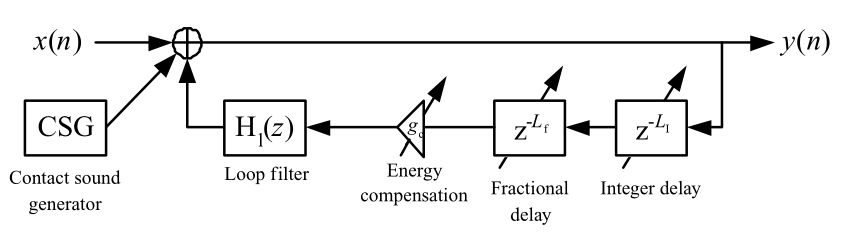
\includegraphics[scale=.75]{./images/pictures/SDL_slide_model.png}
    \caption{Slide guitar DWG model from \citetwo{pakarinen_slide_2008}}
    \label{fig:original_DWG}
\end{figure}

The fundamental control signal for the system is the time-varying relative length of the string, notated as $L[n]$. As shown before, this is what controls the pitch of the synthesized tone. It also controls the sounds generated by the slide/string surface interactions (as will be elaborated upon in Sec.~\ref{sec:CSG_dev}) as the placement of the slide is ultimately what determines the value $L[n]$ takes.

\subsection{Energy Compensation}
Synthesis of slide guitar sounds differs from that of traditional plucked models in that the pitch is a time-varying quantity that does not require another ``pluck" to instantiate the changes. In terms of the DWG model, this translates into a time-varying number of samples for the total DWG length. In order to not have perceptually unnatural shifts in the volume of the synthesized tone, it is necessary to compensate the energy of the signal based on how the string length changes \citetwo{pakarinen_energy_2005}. For instance, if you suddenly move the slide so the relative string length is half of its current value, then half of the samples of the DWG would removed and an unnatural drop in the volume of the sound occurs. Similarly, sliding downwards results in the addition of samples to the DWG which could result in a sudden increase in volume. 

The energy compensation block is what compensates for the string length changes. It is governed by the following equation:
\begin{equation}
    p_c[n] = \sqrt{1-\Delta x}p[n] = g_c p[n]
\end{equation}
where $\Delta x$ is the delay-line variation in samples per one time step, $p[n]$ is the output of the time-varying delay-line, $g_c$ is the scaling coefficient and $p_c[n]$ is the energy compensated signal. This is referred to as zero-order energy-preserving interpolation as is explained in \citetwo{pakarinen_energy_2005}.

\subsection{Loop Filter}
The loop filter is implemented via a single-pole\footnote{\url{https://ccrma.stanford.edu/~jos/filters/Pole_Zero_Analysis_I.html} for information on filter poles as there is too much material to cover here} design with the following transfer-function:

\begin{equation}
    H_l(z) = g \frac{1 + a}{1 + a z^{-1}}
    \label{eqn:one-pole}
\end{equation}
where $a$ controls the cut-off frequency and $g$ controls the gain. $a$ and $g$ determine the characteristics of the tone decay and are meant to model the physical losses associated with string vibration. The parameters were derived from recordings of a professional guitar player playing several notes of every fret for each string in an anechoic chamber. \citetwo{valimaki_development_1998} describes this in more detail.

The $a$ and $g$ parameters are governed by the following first order polynomials:
\begin{align}
    g &= g_{pol}(0) + g_{pol}(1)m_{\text{fret}}\\
    a &= a_{pol}(0) + a_{pol}(1)m_{\text{fret}}\\
    \label{eq:fretNumber}
    m_{fret} &= -12\log_2(L)
\end{align}
where $g_{pol}(n)$ and $a_{pol}(n)$ represent the different polynomial coefficients and $m_{\text{fret}}$ represents the fret number. $m_{\text{fret}}$ is derived from the relative string length based on the rules of the 12-tone equal temperament tuning system. This illustrates how they are interpolated via a first-order polynomial. The polynomial coefficients change for each string and are specified in Table~\ref{tab:g_coeff} and Table~\ref{tab:a_coeff}. Figure~\ref{fig:originalLoopGain} shows the polynomial approximation of $g$ as well as the values extracted from the recordings for the high E string. It is not an exact fit, however it works well enough. Additionally, the plot is specified across the fundamental frequency of the notes which are generated at each different fret number.

\begin{table}[h]
\centering
\begin{tabular}{|c| c| c|} 
 \hline
     & $g_{pol}(0)$ & $g_{pol}(1)$ \\ [0.5ex] 
 \hline
 String 1 & 0.99402123928178  & 0.00008928138142 \\ 
 String 2 & 0.99247813966550  & 0.00012644399078 \\ 
 String 3 & 0.99012478445221  & 0.00025250158133 \\ 
 String 4 & 0.98780640700360  & 0.00037712305083 \\ 
 String 5 & 0.98347976839019  & 0.00040239847018 \\ 
 String 6 & 0.97816203269973  & 0.00061375406757 \\ 
 \hline
\end{tabular}
\caption{Coefficients for first-order polynomial fit to loop-gain data \citetwo{valimaki_development_1998}}
\label{tab:g_coeff}
\end{table}

\begin{table}[h]
\centering
\begin{tabular}{|c| c| c|} 
 \hline
     & $a_{pol}(0)$ & $a_{pol}(1)$ \\ [0.5ex] 
 \hline
 String 1 & -0.02955827361150  & 0.00134421335136 \\ 
 String 2 & -0.03042891937178  & 0.00113090288951 \\ 
 String 3 & -0.03840938807507  & 0.00081125415233 \\ 
 String 4 & -0.06091679973956  & 0.00298025530804 \\ 
 String 5 & -0.05928143968051  & 0.00171045642780 \\ 
 String 6 & -0.08135045114297  & -0.00085796015850 \\ 
 \hline
\end{tabular}
\caption{Coefficients for first-order polynomial fit to filter cut-off frequency \citetwo{valimaki_development_1998}}
\label{tab:a_coeff}
\end{table}

\begin{figure}[h]
    \centering
    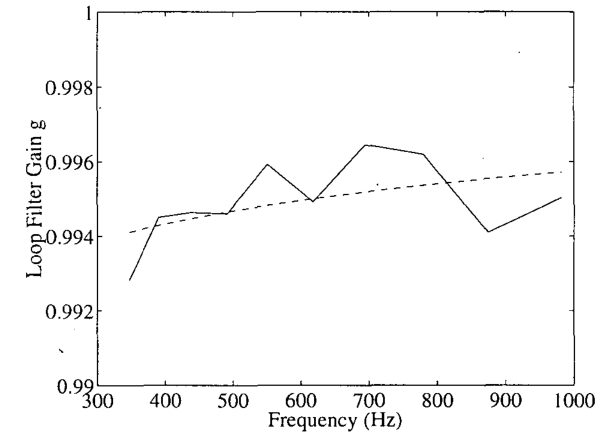
\includegraphics[scale=.75]{./images/plots/Figure18Orig.png}
    \caption{Loop gain $g$ for modeling string 1 (solid line) and first-order polynomial fit (dashed line) as a funciton of frequency. \citetwo{valimaki_development_1998}}
    \label{fig:originalLoopGain}
\end{figure}

\section{CSG Development} \label{sec:CSG_dev}
The handling noises based on wound string and finger interactions have previous been investigated in \citetwo{pakarinen_analysis_2007} and \citetwo{penttinen_model-based_2006}. The slide and string interactions are slightly different, however the underlying framework developed by the finger-noise analysis is valid and the slide synthesis algorithm was adapted from it. In this subsection, the finger-noise analysis will be introduced first followed by the adaptations necessary for the slide scenario.

\subsection{Contact Sound Analysis}
\begin{figure}[h]
    \centering
    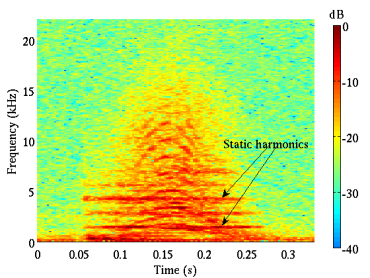
\includegraphics[scale=1]{./images/pictures/finger-noise-spectrogram.png}
    \caption{Spectrogram of handling noise generated by sliding a finger on a wound guitar string from \citetwo{pakarinen_analysis_2007}}
    \label{fig:finger_noise_spectrogram}
\end{figure}

Figure~\ref{fig:finger_noise_spectrogram} shows the spectrogram of the noise generated by dragging a finger tip across the surface of a wound guitar string \citetwo{pakarinen_analysis_2007}. As can clearly be seen, there are two spectral components to the sound. The first is a time-varying harmonic component which corresponds to the interactions of the finger tip with the spatially periodic windings on the string's surface. The second is a static component which is due to the longitudinal modes being stimulated by the finger tip's impacts with the windings. Similar results have been shown in \citetwo{penttinen_model-based_2006} where the guqin, a fretless Chinese stringed instrument using wound strings, was examined.

\subsubsection{Harmonic Component}
An object moving along a wound string creates a harmonic force excitation to the string based on its velocity as well as the texture of the string's surface \citetwo{pakarinen_analysis_2007}. In terms of a finger moving along a wound string, this can mathematically be expressed as:

\begin{equation}
    F_{harm}(t) = \left[\sum_k \delta(t-t_k)\right] \ast f(t)
    \label{eqn:harmonic_force}
\end{equation}
where $f(t)$ is the impulse response from a single finger-winding collision, $t_k$ is the time instant where the $k$th impulse response is generated and $\delta$ is Dirac's delta function. This equation can also be interpreted as a periodic impulse train which is filtered by the transfer function of a single finger-to-winding collision.

To understand how the $t_k$ values are established, lets assume the finger motion is described by a constant velocity. The rate at which winding collisions will occur is a function of the finger velocity as well as linear string winding density. Given that this rate is inversely proportional to $t_k$, the following mathematical expression holds:
\begin{equation}
    t_k = \frac{k}{n_w f_{speed}}
    \label{eqn:t_k}
\end{equation}
where $n_w$ represents the linear winding density of the string (winds per meter) and $f_{speed}$ represents the finger tip speed (meters per second). This means the quantity $n_w f_{speed}$ has units of windings per second and represents the rate of collisions (as alluded to before). By either increasing the linear winding density or finger speed the frequency at which the impulse responses are generated can be controlled. As the $n_w$ parameter is constant for a string, the fundamental frequency of the generated harmonic component is controlled by the speed at which the finger moves. The faster the finger moves, the shorter the time between impacts is and the higher the fundamental of the resulting waveform. A time-varying finger velocity generates a time-varying harmonic signal where the periodic waveform corresponds to the impulse response of a single finger-to-winding impact for that particular string.

This theory can be verified empirically by observing the spectrum in Fig.~\ref{fig:finger_noise_spectrogram}. In the figure, the finger starts at rest and accelerates to reach its maximum velocity halfway through the slide. At this point it begins to decelerate eventually returning to rest once the movement comes to an end. The minimum and maximum values of harmonic frequency trajectories illustrate the same behavior. The harmonics follow a differentiable trajectory. It can be concluded that the finger velocity must also be differentiable, which is useful information when generating control signals for the synthesizer. 

As shown experimentally in \citetwo{pakarinen_analysis_2007}, the amplitude of the harmonic noise component is linearly related to the slide velocity. This can also be intuited from a physical standpoint given that the higher the finger velocity, the more momentum is transferred to the string during the collision. Assuming linearity, this would manifest itself as a velocity dependent scaling component associated with each $t_k$ value in Eq.~\ref{eqn:harmonic_force}.

\subsubsection{Static Component}
The other component from the sound, which has been explicitly labeled in Fig.~\ref{fig:finger_noise_spectrogram}, is are static components due to the longitudinal modes of the string. To understand this, it is necessary to examine the partial differential equation which describes the longitudinal vibrations in a string. As derived in \citetwo{bank_physics-based_2006}, the longitudinal wave equation for a string can be expressed as:
\begin{equation}
    \mu \frac{\partial^2 \xi}{\partial t^2} = ES\frac{\partial^2 \xi}{\partial x^2} - 2R(f)\mu \frac{\partial \xi}{\partial t} + d(x,t)
    \label{eqn:longitudinal_PDE}
\end{equation}
where:
\begin{itemize}
    \item $\xi(x,t)$ is the longitudinal displacement
    \item $E$ is Young's modulus
    \item $S$ is the string's cross sectional area
    \item $\mu$ is the linear mass density
    \item $R(f)$ is a frequency dependent frictional resistance
    \item $d(x,t)$ is the excitation force density
\end{itemize}

For a longitudinal string wave, the propagation speed is $c_L = \sqrt{\frac{ES}{\mu}} = \sqrt{E \rho}$, where $\rho$ is the density of the material. Contrary to transverse modes, the longitudinal propagation speed does not depend on the tension in the string. Suppose that the string is only excited at one spatial location, $x_{exc}$. In this case then the spatial force distribution can be approximated as: $d(x,t) = \delta(x_{exc})F_{exc}(t)$ where $F_{exc}(t)$ is the excitation force applied.

As shown in \citetwo{pakarinen_analysis_2007} and \citetwo{morse_vibration_1981}, for a given $F(t)$ applied at $x_{exc}$, the bridge force can be expressed as:

\begin{equation}
    F_b(t) = \frac{ES}{\mu L^2} \sum_{k = 1}^{\infty} \left[\frac{k}{f_k} e^{-t R(f_k)} \sin(2\pi f_k t)\right] \ast \left[ \sin\left(\frac{k \pi x_{exc}}{L}\right) F_{exc}(t)\right]
    \label{eqn:bridge_force}
\end{equation}
where the longitudinal modal frequencies are $f_k = k \frac{c_L}{2L}$. Equation~\ref{eqn:bridge_force} clearly shows that the force signal excites a set of parallel resonances where the excitation amplitude depends on $x_{exc}$. In general, $x_{exc}$ has a strong shape over the spectrum and in the cases where a mode has a node at the point, the harmonic will be eliminated. This theory was experimentally verified in \citetwo{pakarinen_analysis_2007}. This equation also gives rise to the exciter-resonator perspective as the longitudinal modes can be interpreted as a set of parallel resonances stimulated by an excitation, $F_{exc}(t)$, whose amplitude depends on $x_{exc}$.

\subsection{Adapting From Finger to Slide}
Extrapolating this to the more rigid slide object is rather intuitive. The physical properties of the string do not change, only the surface of the object interacting with the string. In terms of impact on the analysis, the only part of the equations which would change is the impulse response function $f(t)$ in Eq.~\ref{eqn:harmonic_force}. This would now represent the impulse response of a single slide-to-winding impact. All the other analysis applies to a more general model and does not need to change drastically. Additionally, the finger tip velocity should be replaced by the slide velocity.

\subsection{Model Description}
The CSG of the slide synthesis model can be seen as a discretization of the exciter-resonator model developed in the previous section. Figure~\ref{fig:original_CSG} shows a high-level signal flow diagram of the original CSG presented in \citetwo{pakarinen_virtual_2008}. 
\begin{figure}[h]
    \centering
    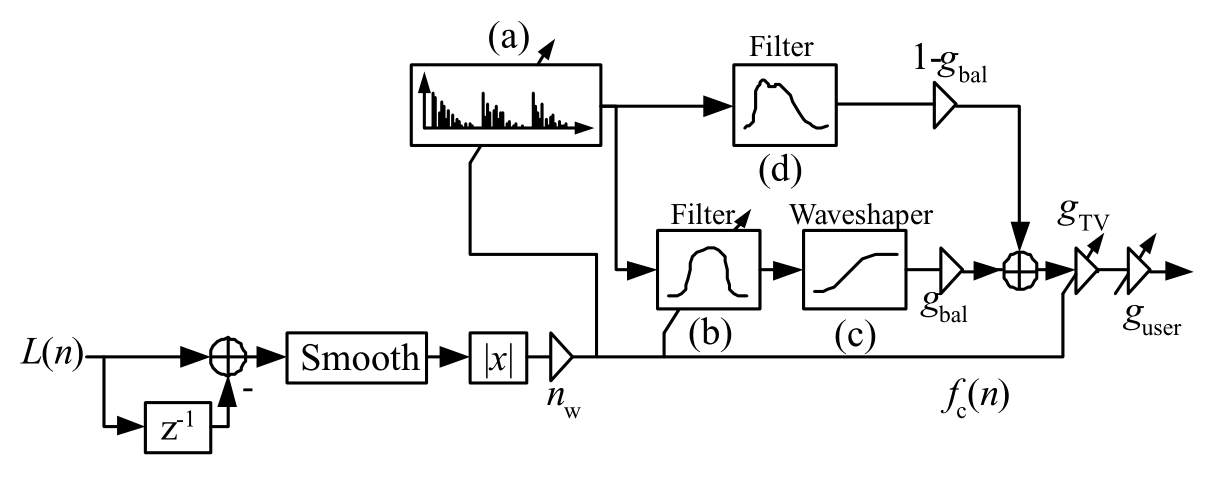
\includegraphics[scale=.50]{./images/pictures/CSG_original.PNG}
    \caption{CSG model from \citetwo{pakarinen_slide_2008}}
    \label{fig:original_CSG}
\end{figure}
A noise pulse train is chosen as the excitation signal (labeled as block $(a)$ in Fig.~\ref{fig:original_CSG}). This choice is based on the assumption that the impulse response from a single slide-to-winding collision can be modeled as an exponentially decaying noise burst. Example noise bursts are shown in Fig.~\ref{fig:noise_pulses_ch2}. The time-interval between noise pulses is controlled by the slide velocity as illustrated in Eq.~\ref{eqn:t_k}. In a certain regard, the CSG can be viewed more as a periodic impact synthesis model more so than a frictional model, which matches with how the slide makes contact with the windings. The faster the slide moves, the denser the pulse train becomes, with some of the IRs overlapping depending on the decay rate associated with the string. The decay rate and correspondingly duration of the noise pulses are parameters associated with each different string thickness. This model is meant to perceptually achieve a similar sound so some theoretical aspects are missing. Contrary to the theory, the location of stimulation does not scale the amplitude of the stimuli. The internals of this module will be elaborated upon in a later chapter.

\begin{figure}[h]
    \centering
    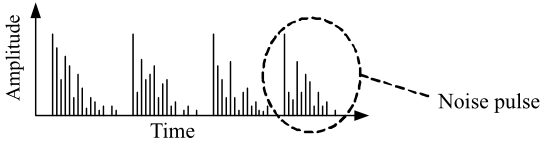
\includegraphics[scale=1]{./images/pictures/noise_pulses.png}
    \caption{Noise Pulses from \citetwo{pakarinen_slide_2008}}
    \label{fig:noise_pulses_ch2}
\end{figure}

At the lower-left branch of the CSG, the control signal $L(n)$ is input. This represents the relative length of the string. The first-order derivative of $L(n)$ is approximated to generate the relative slide-velocity. From there the signal runs through a block labeled ``Smooth" which performs two different operations. The first action is to smooth the input signal to help handle any discontinuities which arise during the differentiation process. A discontinuity in slide-velocity would not be physically possible due to the human controlled nature of the slide motion. The second operation the block performs is interpolation in the case that the control signal runs at a different sampling frequency than the audio signals (as is often the case). The interpolation allows the constituent synthesis model processing blocks to adjust their parameters in a more gradual way as well and mitigates the introduction of transients in digital filters. In this scenario, ultimately a noise-like signal is being filtered so this is not as much of a concern but good to be aware of in general.

After the slide velocity has been up-sampled to the audio rate, the absolute value is then taken to produce the slide speed. Given that the impulse response generated from the impact of the slide with a winding is agnostic to the direction the slide is traveling, this is a valid operation. Subsequently, the relative slide speed is multiplied by $n_w$, the linear winding density, to generate the control signal labeled $f_c(n)$. This signal mimics the relationships expressed in Eq.~\ref{eqn:t_k}. Accordingly, it controls the firing rate of the noise pulse generator as well as scales the output via the gain block $g_{TV}$ to match the amplitude measurements made in \citetwo{pakarinen_analysis_2007}.

The output of the noise pulse generator goes to two different branches, each approximating a different aspect of the contact sound. The lower branch is a 2nd-order resonator filter followed by a waveshaper implemented via a hyperbolic tangent function. The 2nd-order resonator has its center frequency controlled by the aforementioned $f_c(n)$ in order to extract the time-varying fundamental from the harmonic pulse train output. The series connection with the waveshaper creates and accentuates the higher harmonics in a computationally efficient manner. The number of harmonics can be controlled via a scaling factor to the input of the hyperbolic tangent. This is meant to be tuned to match the number of harmonics that have been observed in measurements.

The upper branch serves to emulate the static longitudinal modes using the filter labeled (d). It is a 4th-order IIR which approximates the two most prominent longitudinal modes observed. The coefficients of the filter are dependent on the different string/slide combinations as the different slide materials interact with the windings in a different manner. The filter's responses have been approximated via linear predictive coding (LPC) as described in \citetwo{pakarinen_virtual_2008}. $g_{bal}$ is a scaling coefficient which controls the balance between the longitudinal modes and the harmonic contact sound components.

\subsubsection{Unwound Strings}
Not depicted in Fig.~\ref{fig:original_CSG} is the model which generates the sounds for unwound strings. In this scenario the smooth surface of the slide interacts with the smooth surface of the string, resulting in a pure friction model for the synthesis with no longitudinal component. This can be achieved by replacing block (a) with a white noise generator whose output is scaled by the slide velocity \citetwo{pakarinen_virtual_2008}.

\section{Recent Developments and Approaches}
\citetwo{pakarinen_virtual_2008} is one of the first articles published regarding slide guitar synthesis. There have been refinements and advancements since it was released in 2008. These approaches tend to take a more theoretical approach as compared to the empirical one described in CMJ. The theoretical refinements add computational complexity at the potential cost of a real-time implementation.

\subsection{Evangelista's DWG Approach}
In 2012, Gianpaolo Evangelista published a paper as part of an AES convention which proposes a physically inspired DWG based model \citetwo{evangelista_physical_2012}. His model is a theoretical advancement in many ways, one of which is an expansion in the number of dimensions used to model the vibrations as indicated in Fig.~\ref{fig:EvangelistaCoordinateSystem}. Two DWG structures model the transverse vibrations, one for each of the orthogonal polarizations. Additionally, a DWG is also used to model the longitudinal vibrations as opposed to an IIR filter. This would more accurately model the system and makes the slide's direction important in addition to its speed. The transverse and longitudinal DWGs are weakly coupled in a non-linear fashion at the point where the slide has been placed.

\begin{figure}[h]
    \centering
    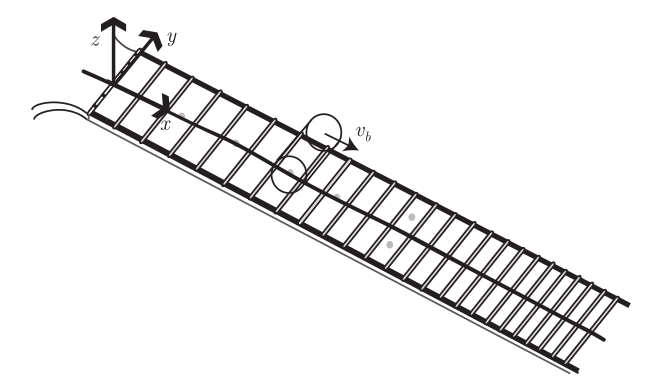
\includegraphics[scale=.65]{./images/diagrams/EvangelistaCoordinateSystem.png}
    \caption{Coordinate system used to describe string and slide motion in Evangelista's approach \citetwo{evangelista_physical_2012}.}
    \label{fig:EvangelistaCoordinateSystem}
\end{figure}

As a basis for the friction sounds, Evangelista uses the Lu-Gre model. The Lu-Gre model only considers flat surfaces interacting and the wound string surface is a violation of this assumption. A new noise term has been added to the model to compensate and this addition is supported by experimental evidence. A non-linear state space model is used to describe the string and Lu-Gre bristle interactions. This produces a single equation which is solved via the Newton-Raphson method. Additionally, the transverse vibrations are taken into account when generating the friction sounds as there is minor interaction between the string and slide at the point of contact. 

A movable slide junction has also been introduction to refine the model further. This is placed at integer string samples and uses fractional delay methods when required. The slide junction models the interactions between the slide and string based on the respective materials of each component. A single parameter is used to control elasticity of the string-winding coefficients on the range from being completely inelastic to elastic. The equations governing the slide/string interactions at each node are non-linear. Figure~\ref{fig:EvangelistaSlideJunction} depicts the slide junction.

\begin{figure}[h]
    \centering
    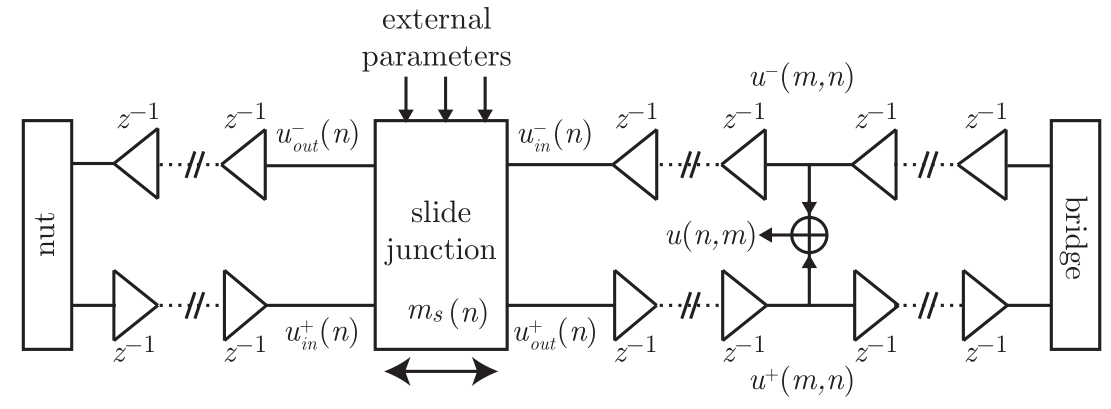
\includegraphics[scale=.5]{./images/diagrams/EvangelistaSlideJunction.png}
    \caption{Slide junction model introduced in \citetwo{evangelista_physical_2012}.}
    \label{fig:EvangelistaSlideJunction}
\end{figure}

A less substantial change is added support for either round-wound or flat-wound strings in the synthesis model by changing the geometry of the string surfaces. There is no mention of the control signal and its characteristics for optimum realism. He makes a claim that this could be run as a real-time model however no evidence is provided to support this. Given that the complexity of the theoretical advancements substantially increase the amount of computation necessary to render a sound, it is questionable if a real-time implementation is possible. Unfortunately sound samples are not included to assess the quality of the results.

\subsection{Belfast Finite-Difference Technique}
The most recent approach to slide guitar synthesis is a finite-difference approach published by a group of researchers at Queen's University Belfast \citetwo{bhanuprakash_finite_2020}. The fundamental approach itself is also a departure from the previous models, as it attempts to numerically simulate the differential equations used to describe the string motion as opposed to simulating the traveling wave variables. By contrast, this is a much more mathematically and computationally intense and does not lend itself easily to real-time synthesis applications. There are also various stability criteria which must be satisfied. The extra complexity is worth it however as the sounds produced are substantially more expressive and realistic. The audio examples can be found at \url{https://abhiram1989.wixsite.com/slidestringfdmodel}.

\begin{figure}[h]
    \centering
    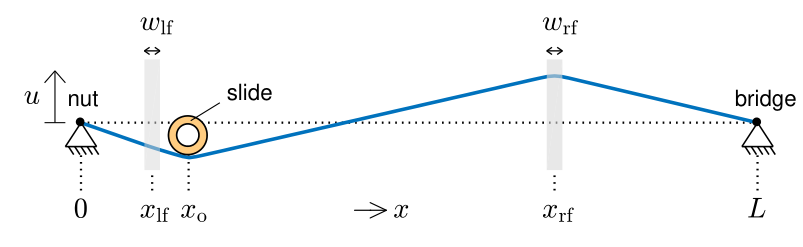
\includegraphics[scale=.75]{./images/diagrams/FDModel.png}
    \caption{Spatial layout for finite difference approach. The gray areas represent finger force regions \citetwo{bhanuprakash_finite_2020}.}
    \label{fig:FDModel}
\end{figure}

In terms of the physical model, advancements have been made to factor in the left and right hand actions. The damping provided by the part of the left-hand behind the slide is explicitly modeled as this is an integral part of the technique involved on a real instrument. The slide attachment/de-attachment sounds are taken into account as these are included within the hand motions. Comparatively speaking the vibration modeling is simpler than Evangelista's or the Finnish approaches. Only one polarization for transverse vibrations is included and the longitudinal vibrations are neglected entirely. Figure~ \ref{fig:FDModel} illustrates the spatial layout of the model.

From a friction standpoint the model used is also lacking as friction is not explicitly modeled (in contrast to the other approaches). However, in the synthesized sounds a noise component can be heard. This is especially true during vibrato sections of phrases. This implies that the sliding noise is not purely based on friction and is likely a mix of friction as well as restoring force-based phenomena which would represent an advancement in the overall knowledge of physics of slide guitar in general.

The control of the model to properly generate realistic and musical sounding results is also a crucial focus of the paper. Four control signals are used in the examples they have provided. These include the slide position, the left hand height, the force applied by the left hand and the force applied by the right hand when plucking. Video footage of expert players was analyzed in an attempt to understand the motions better. Additionally, the researchers attempted to gain an embodied understanding of the motions by learning to play the instrument themselves. The results have paid off as is illustrated by the expressiveness and realism in the synthesized sounds.
\end{document}